\documentclass{scrartcl}
\usepackage{listings}
\usepackage{xcolor}

\definecolor{lightcyan}{HTML}{E0FFFF}
\usepackage[colorlinks=true, urlcolor=blue, linkcolor=red]{hyperref}
\usepackage{graphicx}


\begin{document}
    \lstset{
        language=Java,
        numbers=left,
        stepnumber=1,
        numbersep=5pt,
        backgroundcolor=\color{lightcyan},
        showspaces=false,
        showstringspaces=false,
        showtabs=false,
        tabsize=2,
        captionpos=b,
        breaklines=true,
        breakatwhitespace=true,
        title=\lstname,
    }

\section{Sources}

\begin{itemize}
    \item \url{https://redips789.github.io/spring-certification/Spring-Certification.html}
    \item \url{https://www.baeldung.com/inversion-control-and-dependency-injection-in-spring}
    \item \url{https://www.baeldung.com/inversion-control-and-dependency-injection-in-spring}


    \item \url{https://www.baeldung.com/spring-bean-names}
    \item \url{https://www.baeldung.com/spring-core-annotations}
    \item \url{https://www.baeldung.com/spring-bean-annotations}
    \item \url{https://www.baeldung.com/spring-component-scanning}
    \item \url{https://www.baeldung.com/spring-annotations-resource-inject-autowire}
    \item \url{https://www.digitalocean.com/community/tutorials/spring-bean-life-cycle}
\end{itemize}

TBD
https://www.baeldung.com/spring-annotations-resource-inject-autowire

\section{Dependency injection}
\subsection{Constructor-based}

    In the case of constructor-based dependency injection, the container will invoke a constructor with arguments each representing a dependency we want to set.

    \begin{lstlisting}
        @Configuration
        public class AppConfig {
            @Bean
            public Item item1() {
                return new ItemImpl1();
            }
            @Bean
            public Store store() {
                return new Store(item1());
            }
        }
    \end{lstlisting}

    Resp.

    \begin{lstlisting}
        <bean id="item1" class="org.baeldung.store.ItemImpl1" />
        <bean id="store" class="org.baeldung.store.Store">
        <constructor-arg type="ItemImpl1" index="0" name="item" ref="item1" />
        </bean>
    \end{lstlisting}

\subsection{Setter-based}

    For setter-based DI, the container will call setter methods of our class after invoking a no-argument constructor or no-argument static factory method to instantiate the bean.

    \begin{lstlisting}
        @Bean
        public Store store() {
            Store store = new Store();
            store.setItem(item1());
            return store;
        }
    \end{lstlisting}

    Resp.

    \begin{lstlisting}
        <bean id="store" class="org.baeldung.store.Store">
        <property name="item" ref="item1" />
        </bean>
    \end{lstlisting}

\subsection{Field-based}

    In case of Field-Based DI, we can inject the dependencies by marking them with an @Autowired annotation:

    \begin{lstlisting}
        public class Store {
            @Autowired // deprecated
            private Item item;
        }
    \end{lstlisting}

    Drawbacks:
    \begin{itemize}
        \item This method uses reflection to inject the dependencies, which is costlier than constructor-based or setter-based injection.
        \item It’s easy to keep adding multiple dependencies using this approach. If we were using constructor injection, having multiple arguments would make us think that the class does more than one thing, which can violate the Single Responsibility Principle.
    \end{itemize}

\section{Annotations}
\subsection{Annotations for dependency injection}
\subsubsection{@Autowired}
    @Autowired marks a dependency which Spring is going to resolve and inject. We can use this annotation with a constructor, setter, or field injection. E.g.

    \begin{lstlisting}
        class Car {
            @Autowired
            Engine engine;
        }
    \end{lstlisting}

    Starting with version 4.3, we don’t need to annotate constructors with @Autowired explicitly unless we declare at least two constructors.

\subsubsection{@Bean}

    @Bean marks a factory method which instantiates a Spring bean.

    \begin{lstlisting}
        @Bean
        Engine engine() {
            return new Engine();
        }
    \end{lstlisting}

    Spring calls these methods when a new instance of the return type is required. All methods annotated with @Bean must be in @Configuration classes.

\subsubsection{@Value}

    We can use @Value for injecting property values into beans. It’s compatible with constructor, setter, and field injection. E.g.

    \begin{lstlisting}
        Engine(@Value("8") int cylinderCount) {
            this.cylinderCount = cylinderCount;
        }
    \end{lstlisting}

    This is an alternative to making explicit use of Spring's Environment bean. E.g.

    \begin{lstlisting}
       public DataSource dataSource(
        @Value("${db.driver}") String driver,
        ...
        )
        }
    \end{lstlisting}

\subsubsection{@DependsOn}

    We can use this annotation to make Spring initialize other beans before the annotated one. Usually, this behavior is automatic, based on the explicit dependencies between beans. We only need this annotation when the dependencies are implicit, for example, JDBC driver loading or static variable initialization. E.g.

     \begin{lstlisting}
        @Bean
        @DependsOn("fuel")
        Engine engine() {
            return new Engine();
        }
    \end{lstlisting}

\subsubsection{@Lazy}

    This annotation behaves differently depending on where we exactly place it.

    \begin{itemize}
        \item In an @Bean-annotated bean factory method, it is used to delay the method call (hence the bean creation)
        \item With an @Configuration class, all contained @Bean methods will be affected
        \item For all other @Component classes,  they will be initialized lazily when so annotated.
        \item @Autowired constructors, setters, and fields will be loaded lazily (via proxy).
    \end{itemize}

    \begin{lstlisting}
        @Configuration
        @Lazy
        class VehicleFactoryConfig {

            @Bean
            @Lazy(false)
            Engine engine() {
                return new Engine();
            }
        }
    \end{lstlisting}

\subsubsection{@Scope}

    @Scope is used to define the scope of a @Component class or a @Bean definition. It can be either singleton, prototype, request, session, globalSession or some cust@Component.

\subsection{Context Configuration Annotations}

\subsubsection{@Import}

    We can use specific @Configuration classes without component scanning with this annotation. We can provide those classes with @Import‘s value argument.

    \begin{lstlisting}
        @Import(VehiclePartSupplier.class)
        class VehicleFactoryConfig {}
    \end{lstlisting}

\subsubsection{@ImportResource}

    We can import XML configurations with this annotation. We can specify the XML file locations with the locations argument, or with its alias, the value argument:

    \begin{lstlisting}
        @Configuration
        @ImportResource("classpath:/annotations.xml")
        class VehicleFactoryConfig {}
    \end{lstlisting}

\subsubsection{@PropertySource}

    With this annotation, we can define property files for application settings.

    \begin{lstlisting}
        @Configuration
        @PropertySource("classpath:/annotations.properties")
        @PropertySource("classpath:/vehicle-factory.properties")
        class VehicleFactoryConfig {}
    \end{lstlisting}

    These properties can be used by Spring's Environment bean, in addition to environment variables and Java system properties.

    Allowed prefixes are classpath:, file:, and http:.

\subsection{Bean annotations}

    There are three ways to configure beans:

    \begin{itemize}
        \item XML configuration
        \item Annotation-based, using @Bean
        \item Component scanning, using annotations from org.springframework.stereotype
    \end{itemize}

\subsubsection{@Profile}

    Profiles are a way to group bean definitions, for example:

     \begin{itemize}
        \item dev, test, prod environment
        \item jdbc, jpa [implementations]
    \end{itemize}

   The @Profile annotation may be used in any of the following ways:

   \begin{itemize}
       \item At class level in @Configuration classes.
       \item At class level in classes annotated with @Component or annotated with any other annotation that in turn is annotated with @Component.
       \item On methods annotated with the @Bean annotation.
   \end{itemize}

    To define alternative beans with different profile conditions, use distinct Java method names pointing to the same bean name via the @Bean name attribute:

    \begin{lstlisting}
        @Bean("dataSource")
        @Profile("development")
        public DataSource standaloneDataSource(){

        @Bean("dataSource")
        @Profile("production")
        public DataSource jndiDataSource() throws Exception {}

    \end{lstlisting}

   Spring uses two separate properties when determining which profiles are active, spring.profiles.active and spring.profiles.default:

    \begin{itemize}
       \item If spring.profiles.active is set,  then its value determines which profiles are active.
       \item If spring.profiles.active isn’t set, then Spring looks to spring.profiles.default.
       \item If neither spring.profiles.active nor spring.profiles.default is set, only those beans that aren’t defined as being in a profile are created.
    \end{itemize}

   These properties can be set on the command line:

   \begin{lstlisting}[language=bash]
       -Dspring.profiles.active=embedded.jpa
   \end{lstlisting}

   , programmatically:

   \begin{lstlisting}
       System.setProperty("spring.profiles.active", "embedded.jpa");
   \end{lstlisting}

   , or via an annotation (@ActiveProfiles; integration tests only).


\subsubsection{@ComponentScan}

    @ComponentScan configures which packages to scan for classes with annotation configuration. E.g., specifying packages:

    \begin{lstlisting}
        @Configuration
        @ComponentScan(basePackages = "com.baeldung.annotations")
        class VehicleFactoryConfig {}
    \end{lstlisting}

    Or else, specifying classes:

    \begin{lstlisting}
        @Configuration
        @ComponentScan(basePackageClasses = VehicleFactoryConfig.class)
        class VehicleFactoryConfig {}
    \end{lstlisting}

    The @ComponentScan annotation is used together with @Configuration.

\subsubsection{@ComponentScan Without Arguments}

    @ComponentScan without arguments tells Spring to scan the current package and all of its sub-packages.

\subsubsection{@ComponentScan With Arguments}

    Passing basePackages, we can, for example, change the base package.

    \begin{lstlisting}
        @ComponentScan(basePackages = "com.baeldung.componentscan.springapp.animals")
        @Configuration
        public class SpringComponentScanApp {
            // ...
        }
    \end{lstlisting}

    Or we can specify multiple package names, using spaces, commas, or semicolons as a separator.

    \begin{lstlisting}
        @ComponentScan(basePackages = "com.baeldung.componentscan.springapp.animals;com.baeldung.componentscan.springapp.flowers")
        @ComponentScan(basePackages = "com.baeldung.componentscan.springapp.animals,com.baeldung.componentscan.springapp.flowers")
        @ComponentScan(basePackages = "com.baeldung.componentscan.springapp.animals com.baeldung.componentscan.springapp.flowers")
    \end{lstlisting}

    We can also apply a filter, choosing from a range of filter types. For example:

    \begin{lstlisting}
        @ComponentScan(excludeFilters =
        @ComponentScan.Filter(type=FilterType.REGEX,
        pattern="com\\.baeldung\\.componentscan\\.springapp\\.flowers\\..*"))
    \end{lstlisting}

    Or:
    \begin{lstlisting}
        @ComponentScan(excludeFilters =
        @ComponentScan.Filter(type = FilterType.ASSIGNABLE_TYPE, value = Rose.class))
    \end{lstlisting}

\subsubsection{@Component}

    @Component is a class-level annotation. During the component scan, Spring Framework automatically detects classes annotated with @Component.

    \begin{lstlisting}
        @Component
        class CarUtility {
            // ...
        }
    \end{lstlisting}

    @Repository, @Service, @Configuration, and @Controller are all meta-annotations of @Component. Spring also automatically picks them up during the component scanning process.

\subsubsection{@Repository}

    \begin{lstlisting}
        @Repository
        class VehicleRepository {
            // ...
        }
    \end{lstlisting}

\subsubsection{@Service}

    \begin{lstlisting}
        @Service
        public class VehicleService {
            // ...
        }
    \end{lstlisting}

\subsubsection{@Controller}

    \begin{lstlisting}
        @Controller
        public class VehicleController {
            // ...
        }
    \end{lstlisting}

\subsubsection{@Configuration}

    Configuration classes can contain bean definition methods annotated with @Bean.

    \begin{lstlisting}
        @Configuration
        class VehicleFactoryConfig {

            @Bean
            Engine engine() {
                return new Engine();
            }

        }
    \end{lstlisting}


\subsection{Spring Boot Annotations}
\subsubsection{@SpringBootApplication}

    This is a combination of three annotations:

    \begin{lstlisting}
        @Configuration
        @EnableAutoConfiguration
        @ComponentScan
    \end{lstlisting}

\subsection{Comparing @Resource, @Autowired, and @Inject annotations}
\subsubsection{@Resource}

    The @Resource annotation matches by name, type, or qualifier (in this order). It is applicable to setter and field injection.
    Here’s an example injecting a field. Note that the bean id and the corresponding reference attribute value must match:

    \begin{lstlisting}
        @Configuration
        public class MyAppContext {
            @Bean(name="namedFile")
            public File namedFile() {
                File namedFile = new File("namedFile.txt");
                return namedFile;
            }
        }

        @ContextConfiguration(
        loader=AnnotationConfigContextLoader.class,
        classes= MyAppContext.class)
        public class Xxx {
            @Resource(name="namedFile")
            private File defaultFile;
        }
    \end{lstlisting}

\subsubsection{@Inject}

    The @Inject annotation matches by type, qualifier, or name (in this order). It is applicable to setter and field injection. With @Inject, the class reference variable name and the bean name don’t have to match.

    To use the @Inject annotation, declare the javax.inject library as a Gradle or Maven dependency.

    \begin{lstlisting}
        public class MyAppContext {
            @Bean
            // no bean name specified - method name is used
            public File getSomeFile() {
                File namedFile = new File("namedFile.txt");
                return namedFile;
            }
        }

        @ContextConfiguration(
        loader=AnnotationConfigContextLoader.class,
        classes= MyAppContext.class)
        public class Xxx {
            @Inject
            private File defaultFile;
        }
    \end{lstlisting}

\subsubsection{@Autowired}

TBD

\section{Aware Interfaces}

    Indicates that the bean is eligible to be notified by the Spring container through the callback methods.
    The typical use case for BeanNameAware could be acquiring the bean name for logging or wiring purposes. For the BeanFactoryAware it could be the ability to use a spring bean from legacy code.
    In most cases, we should avoid using any of the Aware interfaces, unless we need them. Implementing these interfaces will couple the code to the Spring framework.

\subsection{BeanNameAware}

    Makes the object aware of the bean name defined in the container.

\begin{lstlisting}
    public class MyBeanName implements BeanNameAware {
        @Override
        public void setBeanName(String beanName) {
            System.out.println(beanName);
        }
    }
    @Configuration
    public class Config {
        @Bean(name = "myCustomBeanName")
        public MyBeanName getMyBeanName() {
            return new MyBeanName();
        }
    }
    AnnotationConfigApplicationContext context
    = new AnnotationConfigApplicationContext(Config.class);
    MyBeanName myBeanName = context.getBean(MyBeanName.class);

\end{lstlisting}

\subsection{BeanFactoryAware}

    Provides access to the BeanFactory which created the object.

    \begin{lstlisting}
        public class MyBeanFactory implements BeanFactoryAware {
            private BeanFactory beanFactory;
            @Override
            public void setBeanFactory(BeanFactory beanFactory) throws BeansException {
                this.beanFactory = beanFactory;
            }
            public void getMyBeanName() {
                MyBeanName myBeanName = beanFactory.getBean(MyBeanName.class);
                System.out.println(beanFactory.isSingleton("myCustomBeanName"));
            }
        }
        MyBeanFactory myBeanFactory = context.getBean(MyBeanFactory.class);
        myBeanFactory.getMyBeanName();}
    \end{lstlisting}

\subsection{ApplicationContextAware}
    \begin{lstlisting}
        public class ApplicationContextAwareImpl implements ApplicationContextAware {
            @Override
            public void setApplicationContext(ApplicationContext applicationContext) throws BeansException {
                User user = (User) applicationContext.getBean("user");
                System.out.println("User Id: " + user.getUserId() + " User Name :" + user.getName());}}
    \end{lstlisting}

\section{Bean Lifecycle}
\subsection{Overview}

    \begin{figure}
        \centering
        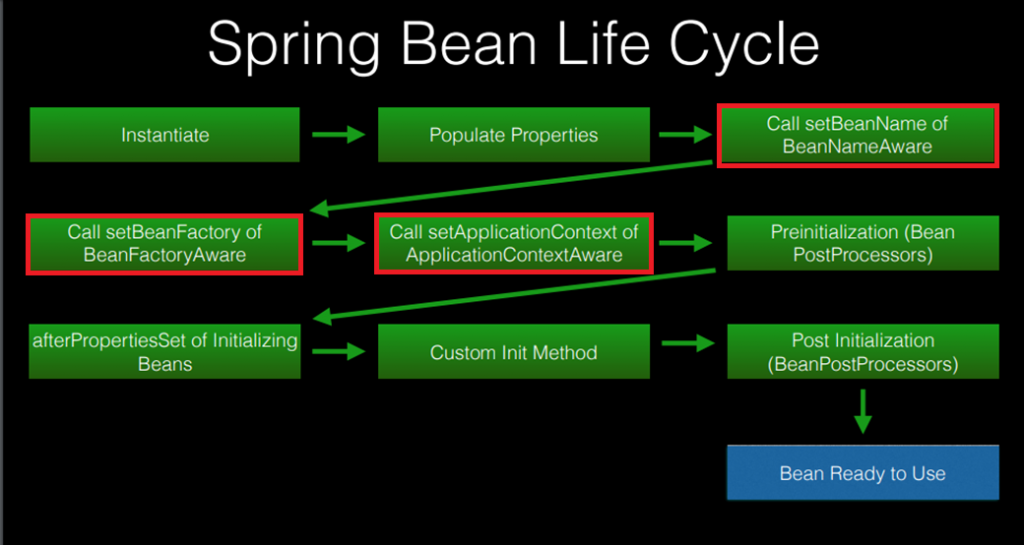
\includegraphics[width=1\linewidth]{bean-lifecycle-1}
        \caption{}
        \label{fig:bean-lifecycle-1}
    \end{figure}

    Zooming in on the pre-instantation changes:

    \begin{figure}
        \centering
        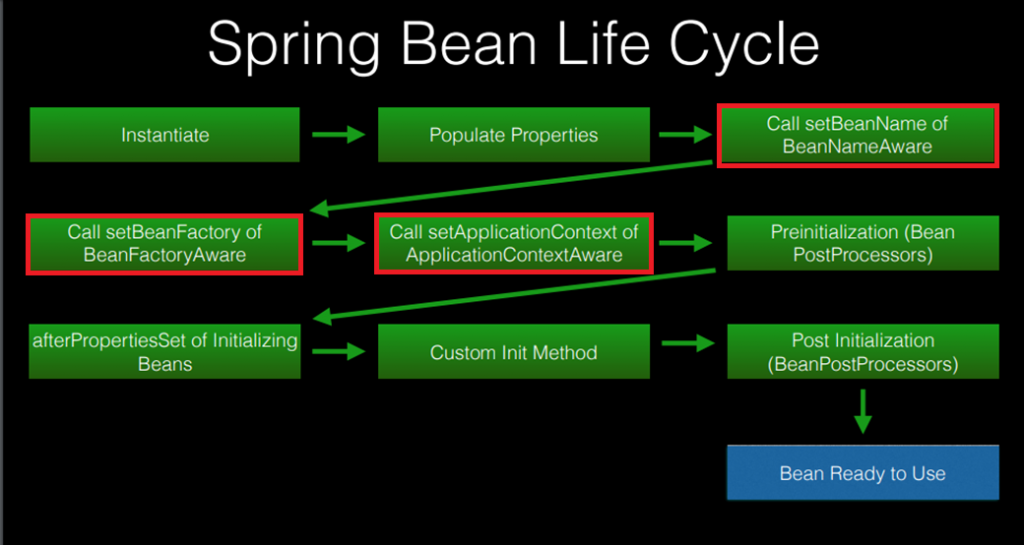
\includegraphics[width=1\linewidth]{bean-lifecycle-1}
        \caption{}
        \label{fig:bean-lifecycle-2}
    \end{figure}

    See https://www.digitalocean.com/community/tutorials/spring-bean-life-cycle for code to display the order of invocations.

\subsubsection{Load bean definitions, creating an ordered graph}
    In this step, all the configuration files – @Configuration classes or XML files – are processed. For annotation-based configuration, all the classes annotated with @Components are scanned to load the bean definitions.
\subsubsection{Instantiate and run BeanFactoryPostProcessors}
    In a Spring application, a BeanFactoryPostProcessor can modify the definition of any bean.
    The BeanFactory object is passed as an argument to the postProcess() method of the BeanFactoryPostProcessor. BeanFactoryPostProcessor then works on the bean definitions or the configuration metadata of the bean before the beans are actually created.
    Spring provides several useful implementations of BeanFactoryPostProcessor, such as reading properties and registering a custom scope. We can write your own implementation of the BeanFactoryPostProcessor interface. To influence the order in which bean factory post processors are invoked, their bean definition methods may be annotated with the @Order annotation. If you are implementing your own bean factory post processor, the implementation class can also implement the Ordered interface.

    \begin{figure}
        \centering
        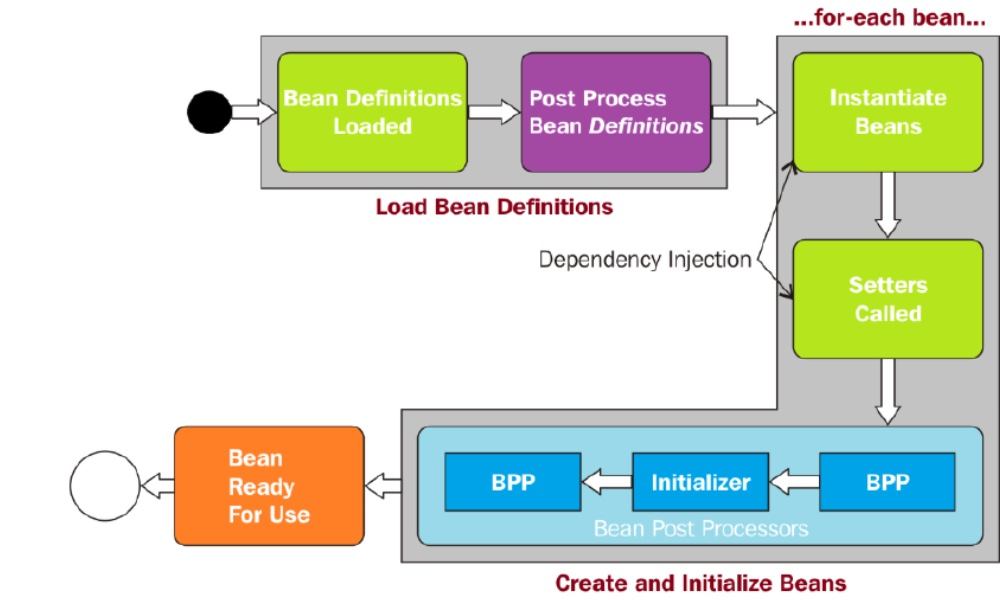
\includegraphics[width=1\linewidth]{bean-lifecycle-3}
        \caption{}
        \label{fig:bean-lifecycle-1}
    \end{figure}

\subsubsection{Instantiate beans}
    Injects values and bean references into beans’ properties.

\subsubsection{Call BeanNameAware’s setBeanName() for each bean implementing it}

\subsubsection{Call BeanFactoryAware’s setBeanFactory() passing the bean factory for each bean implementing it}

\subsubsection{Call ApplicationContextAware’s setApplicationContext for each bean implementing it}

\subsubsection{Run pre-initialization BeanPostProcessors}
    The Application context calls postProcessBeforeInitialization() for each bean implementing BeanPostProcessor.
    A bean implementing BeanFactoryPostProcessor is called when all bean definitions have been loaded, but no beans will have been instantiated yet. This allows for overriding or adding properties even to eager-initializing beans. This will let you have access to all the beans that you have defined in XML or that are annotated (scanned via component-scan).

\subsubsection{Call InitializingBean’s afterPropertiesSet()}
    If a bean implements the InitializingBean interface, Spring calls its afterPropertiesSet() method. Used to initialize processes,  load resources, etc. This approach is simple to use but it’s not recommended because it will create tight coupling with the Spring framework in our bean implementations.

\subsubsection{Init Method}
    Instead of implementing InitializingBean, you can use the init-method of the bean tag, the initMethod attribute of the @Bean annotation, and JSR 250's @PostConstruct  annotation.
    Here we use the init-method attribute:

    \begin{lstlisting}
        <bean name="myEmployeeService" class="com.journaldev.spring.service.MyEmployeeService"
        init-method="init" destroy-method="destroy">
        <property name="employee" ref="employee"></property>
        </bean>
    \end{lstlisting}


    And here, the @PostConstruct annotation.

    \begin{lstlisting}
        @PostConstruct
        public void init(){
            System.out.println("MyService init method called");
        }
    \end{lstlisting}


\subsubsection{Run post-initialization BeanPostProcessors}
The application context calls postProcessAfterInitialization() for each bean implementing BeanPostProcessor.

\subsubsection{Bean ready to use}
Your beans remain live in the application context until it is closed by calling the close() method of the application context.

\subsubsection{Custom destruction}
If a bean implements the DisposableBean interface, Spring calls its destroy() method to destroy any process or clean up the resources of your application. There are other methods to achieve this step-for example, you can use the destroy-method of the tag, the destroyMethod attribute of the `@Bean` annotation, and JSR 250's `@PreDestroy` annotation.


\section{Bean Naming}
\subsection{Default Bean Naming}
\subsubsection{Class-level}
For an annotation used at the class level, Spring uses the class name and converts the first letter to lowercase.
The same default naming strategy is applicable for all class-level annotations that are used to create a Spring bean, such as @Component, @Service, and @Controller.

    \begin{lstlisting}
        @Service
        public class LoggingService { // bean name = loggingService

        }
    \end{lstlisting}

\subsubsection{Method-level}
When we use the @Bean annotation on a method, Spring uses the method name as a bean name.

    \begin{lstlisting}
        @Configuration
        public class AuditConfiguration {
            @Bean
            public AuditService audit() {
                return new AuditService();
            }
        }
    \end{lstlisting}

\subsection{Custom naming}

    \begin{lstlisting}
        @Component("myBean")
        public class MyCustomComponent {
        }
    \end{lstlisting}

    Similar to @Component(“myBean”), we can specify the name using other annotations such as @Service(“myService”), @Controller(“myController”), and @Bean(“myCustomBean”).

\subsection{Naming Beans With @Bean and @Qualifier}
\subsubsection{@Bean With Value}
    The @Bean annotation is applied at the method level, and by default, Spring uses the method name as a bean name. We can override this using the @Bean annotation.

     \begin{lstlisting}
        @Configuration
        public class MyConfiguration {
            @Bean("beanComponent")
            public MyCustomComponent myComponent() {
                return new MyCustomComponent();
            }
        }
    \end{lstlisting}

\subsubsection{@Qualifier With Value}
    We can also use the @Qualifier annotation to name the bean.

    \begin{lstlisting}
        @Component
        @Qualifier("cat")
        public class Cat implements Animal {
            @Override
            public String name() {
                return "Cat";
            }
        }
        @Component
        @Qualifier("dog")
        public class Dog implements Animal {
            @Override
            public String name() {
                return "Dog";
            }
        }
        @Service
        public class PetShow {
            private final Animal dog;
            private final Animal cat;

            public PetShow (@Qualifier("dog")Animal dog, @Qualifier("cat")Animal cat) {
                this.dog = dog;
                this.cat = cat;
            }
            public Animal getDog() {
                return dog;
            }
            public Animal getCat() {
                return cat;
            }
        }
        \end{lstlisting}

\end{document}




























